\chapter{Fundamentação Teórica}
\label{ch:fundamentos}

Neste capítulo são abordados conceitos importantes para o entendimento das técnicas que são utilizadas neste trabalho. A Seção \ref{sec:evolutionary_algorithms} é introduzido os algoritmos evolutivos, apresentando seus pontos fortes e suas influências para a otimização de problemas complexos. A seguir, na Seção \ref{sec:swarm_intelligence_algorithms} é introduzido os algoritmos de inteligência de enxame e seus pontos positivos na otimização de problemas dinâmicos. Por fim, na Seção \ref{sec:intesification_diversification} é apresentado a relação de intensificação e diversificação na convergência de algoritmos durante o processo de otimização.

\section{Algoritmos Evolutivos}
\label{sec:evolutionary_algorithms}
A natureza é uma fonte de inspiração para o desenvolvimento de vários algoritmo, como por exemplo os algoritmos evolutivos. A Computação Evolutiva se inspira no processo da seleção natural e evolução natural. 
Em termos gerais,um algoritmo evolucionário possui alguns componentes básicos para resolução de problemas \cite{parpinelli2011new}

\begin{enumerate}
\item Várias representações para a possíveis soluções do problema;
\item Um modo de criar uma população inicial (aleatório ou determinístico);
\item Uma função que avalia a qualidade das soluções, ou seja, a aptidão do indivíduo (\textit{Fitness});
\item Um mecanismo de seleção para cruzamento;
\item Operadores evolutivos para criação de novas gerações (como mutação e \textit{crossover});
\item Parâmetros para controle do comportamento do algoritmo, como número de dimensões, controle de operadores e etc.  
\end{enumerate}

Nas subsecções estão apresentados os algoritmos do estado da arte que serão utilizados neste trabalho.

\subsection{Algoritmo Genético}
\label{sec:genetic_algorithms}
O Algoritmo Genético (\textit{Genetic Algorithm} - GA) foi um dos primeiro algoritmos bioinspirados a serem propostos durante a década de 60 e 70, ele foi desenvolvido por Holland e seus colaboradores que tem como base a teoria da evolução de Darwin \cite{ga} e é um dos algoritmos mais utilizados na Computação Evolutiva. A seleção natural de Darwin diz que o melhor indivíduo em uma determinada população, tem maiores chances de sobreviver e assim passar sua carga genética adiante, tornado assim a espécie mais apta às condições do ambiente. O GA utiliza essa seleção do indivíduo mais adaptado para direcionar a busca em direção das soluções ótimas.

A otimização do GA começa com a inicialização da população inicial, sendo de forma aleatória ou determinística, em que cada indivíduo possuí um cromossomo, que por sua vez representa uma possível solução para o problema. A partir dessa população inicia-se o primeiro ciclo evolutivo, em que cada indivíduo é avaliado, gerando assim um valor de aptidão (\textit{fitness}) para ser usado na seleção da população. A seleção determina quais indivíduos irão cruzar gerando uma população intermediária, de modo que os mais adaptados tenham uma maior chance de serem selecionados. Os operadores evolutivos de cruzamento e mutação, são aplicados na população intermediária, em que o cruzamento tem o papel de intensificar a busca e a mutação o de diversificar a população. A partir deste ciclo o algoritmo se repete até que o critério de parada seja satisfeito, aplicando cada ciclo na população gerada pelo ciclo anterior.

\subsection{Evolução Diferencial}
\label{sec:diferencial_evolution}
A evolução diferencial (\textit{Diferencial Evolution} - DE) e uma meta-heurística evolucionária para otimização de funções contínuas, proposta por Storn e Price em 1995 \cite{de}. Seu nome se dá pela sua rotina de mutação que acontece por uma operação de subtração (diferenciação). O DE é amplamente estudado e as características que o tornam interessante são: Sua simplicidade, pois é um algoritmo com poucos operadores evolutivos e simples de serem implementados; Seu bom desempenho, tendo uma convergência rápida o DE se destaca entre vários outros algoritmos evolutivos; e pelo fato de possuir poucos parâmetros, tornando assim sua aplicação mais fácil e intuitiva.

O DE possui, basicamente, uma etapa de inicialização e três etapas em seu ciclo de evolução: mutação, cruzamento e seleção (nessa ordem). O processo evolutivo é iniciado após a inicialização do algoritmo e é finalizado quando um determinado critério de parada for atingido. Primeiramente, o usuário define o tamanho da população ($\lambda$), taxa de chance de \textit{crossover} ($C_r$) e fator de escala ($F$). Existem três tipos de vetores no DE que são: Vetor alvo, que é o vetor pai da geração atual; O vetor doador, que é gerado à partir da mutação; e o vetor \textit{trial}, que é a combinação do vetor alvo com o vetor doador gerado pelo cruzamento. 

Para criar o vetor doador, obtém-se uma amostra de três indivíduos distintos na população, assim é criado uma mutação à partir da diferença de dois destes vetores, multiplicada pelo fator de escala $F$ e somada ao terceiro vetor. A etapa de mutação, responsável pela busca global do algoritmo (diversificação), e é o principal fator caracterizante do DE. O $C_r$ controla o cruzamento que é responsável pela intensificação da busca e acontece à partir da recombinação dos vetores alvo e doador. Ao final a seleção acontece verificando uma melhora no \textit{fitness} do vetor \textit{trial} em relação ao alvo, caso não aconteça uma melhora a nova solução é descartada.

\section{Algoritmos de Inteligência de Enxame}
\label{sec:swarm_intelligence_algorithms}
Os algoritmos de inteligência de enxame
%falar sobre as dificuldades dos problemas de swarm em problemas dinâmicos \cite{blackwell2005particle}:
%- Memória do algoitmo: pois após uma mudança no ambiente, os dados colhetados podem não ser mais válidos falar do "Melhor erro Antes da Mudança"
%- perda de divercidade: 

\subsection{Otimização por Enxame de Partículas}
\label{sec:particle_swarm_optimization}
A otimização por enxame de partículas (\textit{Particle Swarm Optimization} - PSO) foi proposta por Kennedy \cite{pso}. O PSO tem como inspiração o comportamento coordenado dos movimentos dos pássaros e cardumes de peixes. Cada partícula é uma solução potencial para o problema, representada por sua velocidade, localização no espaço de busca e uma memória que armazena a sua melhor posição visitada. O movimento de cada partícula depende de sua própria velocidade e da localização das boas soluções encontradas. O equilibro entre a intensificação e a diversificação é alcançada no PSO através do peso da inércia.

\subsection{Otimização por Colônia de Bactérias}
\label{sec:biomimicry_bacterial_foraging}
O algoritmo de Otimização por Colônia de Bactérias (\textit{Bacterial Foraging Optimization} - BFO) foi proposto por Passino \cite{passino2002biomimicry}, inspirada no comportamento social de busca por alimento das bactérias Escherichia Coli. Durante o processo de busca a bactéria se move em pequenos passos enquanto procura alimento. Seu movimento é realizado através de um conjunto de filamentos conhecido como flagelos, que ajudam a bactéria se mover em períodos alternados de natação (\textit{swim}) e tombos (\textit{tumble}). A alternância entre estes dois períodos chama-se quimiotaxia. Cada bactéria representa uma solução para o problema. O ambiente fornece o substrato para as bactérias interagirem e é representado pelo espaço de busca sendo otimizado. Quanto melhor for a região do espaço de busca, melhor será o resultado da função objetivo, e consequentemente, melhor será o substrato para as bactérias.

O BFO é composto por três rotinas principais: quimiotaxia, reprodução e eliminação-dispersão. Na quimiotaxia, uma bactéria com direção aleatória representa um tombo e uma bactéria com a mesma direção do passo anterior indicando uma execução. Na reprodução, a saúde de cada bactéria representa seu valor de \textit{fitness}. Todas as bactérias são classificadas de acordo com seu estado de saúde e apenas a primeira metade da população sobrevive. As bactérias sobreviventes são divididos em dois filhos idênticos, de modo a formar uma nova população. O processo de eliminação-dispersão é responsável por aumentar a diversidade da população. A dispersão ocorre depois de um certo número de etapas de reprodução, quando algumas bactérias são escolhidos de acordo com uma probabilidade predefinida. Tais bactérias são mortas e os novos são gerados aleatoriamente em outra posição dentro do espaço de busca. A intecificação busca é realizado por ambos os passos de quimiotaxia e de reprodução.

\subsection{Otimização por Colônia Vaga-lumes}
\label{sec:firefly_algorithm}
O algoritmo de Otimização por Colônia de Vaga-Lumes (\textit{firefly algorithm} - FA) por Yang \cite{firefly}. O FA trabalha com 3 regras principais para a otimização de funções \textit{benchmarks}, sendo elas:

\begin{itemize}
\item Um vaga-lume será atraído pelo outro não importando o sexo deles.

\item A atratividade entre dois vaga-lumes aumenta em relação a intensidade do brilho e decresce em relação ao aumento da distância entre eles.

\item A proximidade do vaga-lume em relação a uma solução do espaço de busca influência na intensidade do brilho do mesmo.
\end{itemize}

Cada agente brilha proporcionalmente à qualidade da sua solução que, juntamente com a sua atratividade ($\beta$), ditam o quão forte ela atrai outros membros do enxame. Dois outros parâmetros definidos pelo usuário são o valor máximo de atração ($\beta_i$) e do coeficiente de absorção ($\Upsilon$), que determina a variação de atratividade com o aumento da distância da comunicação dos vaga-lumes. A variável
de intensidade da luz $\beta_i$ de cada vaga-lume, mantém o balanço entre a intensificação e diversificação da busca.

\subsection{Otimização por Colônia de Morcegos}
\label{sec:bat_algorithm}
O algoritmo de Otimização por Colônia de Morcegos foi apresenta pela primeira vez por Yang \cite{bat}. Aplicado aos mesmos \textit{benchmarks} pode-se notar uma desempenho melhor do que os encontrados em AGs e ao PSO. 

A ideia do algoritmo de morcegos é uma população de morcegos (possíveis soluções), em que é usado eco-localização dos morcegos, utilizado durante o seu voo para detectar presas e evitar obstáculos e uma rotina de voo aleatório para movimentação no espaço de busca, atualizando suas posições e suas velocidades. outros parâmetros são: o fator de decaimento de sonoridade ($\alpha$) que atua em um papel semelhante a temperatura do \textit{simulated annealing}, e o fator de aumento de pulso ($\gamma$) que regula a frequência de pulso. A atualização da taxa de pulso ($R_i$) e sonoridade ($A_i$) equilibra o comportamento intensificação e diversificação de cada morcego, respectivamente. De acordo com a diminuição da sonoridade ao morcego encontrar uma presa (solução ótima), a taxa de pulso vai aumentando para melhorar a acurácia do ataque. 

\subsection{Algoritmo de Busca por Cardume de Peixes}
\label{sec:fish_school_search}
O algoritmo de Busca por Cardume de Peixes (\textit{Fish School Search} - FSS) foi proposto por Carmelo \cite{carmelo2008novel}. O processo de pesquisa do FSS é feito por uma população de indivíduos, com memória limitada, representado o peixe. O ambiente de busca é representado pelo mar em que os peixes se encontram, onde eles podem se movimentar para tentar melhorar sua solução. A densidade de comida representa a qualidade da solução, de forma que em um problema de maximização a densidade de comida é diretamente proporcional a qualidade do resultado. A densidade de comida de um local influencia o peixe através do peso, de forma que uma melhora continua da solução apresenta um peixe mais pesado.

\subsubsection{Operadores Evolutivos}
\label{sec:evolutionary_operators}
A versão do algoritmo estuda possui 4 operadores com suas funções bem definidas, que podem ser separados em duas classes \cite{c2009influence}: Alimentação (OA) e Movimentação. Para a movimentação temos as seguintes classificações: Operador de Movimento Individual (OMI); Operador de Movimentação Coletiva Instintiva (OMCI); e Operador de Movimentação Coletiva Volátil (OMCV).

\noindent \textbf{Operador de Movimento Individual}

Este OMI representa o movimento de cada um dos peixes individualmente, sem a influência do cardume. A próxima posição (candidata) é determinada pela geração de um número aleatório, de uma distribuição normal, e esse número é atribuído a uma das posições vizinhas do indivíduo. Após Isso o número é multiplicado por uma variável chama de $Step_ind$, que é a percentagem da amplitude do espaço de busca, essa variável decresce linearmente durante cada iteração, como mostrado na Equação \ref{eq:individual_moviment}.

\begin{equation}
\label{eq:individual_moviment}
\begin{split}
& n_i(t) = x_i(t) + N(-1,1).Step_ind \\
& \Delta f = f(\vec{n}) - f(\vec{x}) \\
& \Delta x = \vec{n} - \vec{x} \\
& Step_ind(t+1) = Step_ind(t) - \frac{Step_indInicial - Step_indFinal}{iteracoes};
\end{split}
\end{equation}

\noindent Em que $n_i$ é a nova posição candidata, $x_i$ é a posição atual, $\Delta f$ é a variação do \textit{fitness} e o $\Delta x$ a variação do movimento. A nova posição é efetivamente atualizada, somente se, ela for melhor que a posição anterior do indivíduo. Sendo assim, pode-se observar que esse operador tem influência na busca global feita por cada indivíduo.

\noindent \textbf{Operador de Alimentação}

Quando são gerados, peixes possuem o mesmo peso, e ao longo da busca esse peso é alterado de acordo com o melhoramento da solução, ou seja, caso a solução melhore o peso aumenta. O peso de cada peixe representa o quão bem o indivíduo está na busca da solução. O cálculo do peso tem influência da população, utilizando maior variação de fitness encontrada entre todos os indivíduos como $\max{\Delta f}$, sendo a diferença entre o melhor e o pior indivíduos, mostrado na Equação \ref{eq:food_operator}.

\begin{equation}
\label{eq:food_operator}
W_i(t+1) = W_i(t) + \frac{\Delta t}{\max{\Delta t}}
\end{equation}

\noindent \textbf{Operador de Movimentação Coletiva Instintiva}

Somente os indivíduos que realizaram o OMI, ou seja, $\Delta x$ tem que ser diferente de zero, terão influência no cálculo do movimento coletivo. Após o calculo todos os indivíduos são atualizados, mesmo os que não realizaram o movimento individual. Esse operador coletivo instintivo tem como contribuição a busca local fazendo com que a população inteira se direcione para um espaço de busca possivelmente melhor, simulando assim, o efeito de um cardume de peixes como pode ser visto da Figura \ref{fig:coletive_moviment}.

\begin{figure}[!htb]
	\caption{Representação gráfica da influência do Movimento Coletivo Instintivo na população}
	\centering
	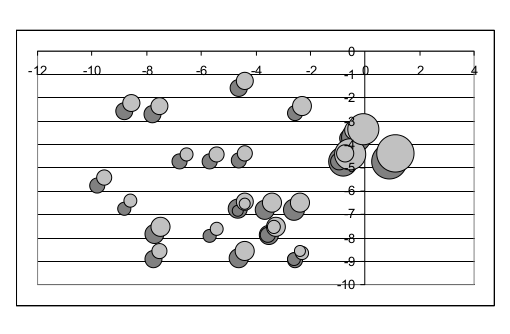
\includegraphics[scale=0.5]{images/movimento_coletivo.png}
	\label{fig:coletive_moviment}{\\Fonte: \citeonline{c2009influence}.}
\end{figure}

\noindent \textbf{Operador de Movimentação Volátil Coletiva}

Este movimento é baseado na melhora em geral da população, que é representada através do peso médio da população. Quando tem-se uma melhora nas soluções ocorre a contração da população em relação ao baricentro dos indivíduos, caso contrário, ocorre a dilatação. O cálculo deste baricentro é feito com base na posição de cada indivíduo e o peso de cada um deles. Todos os indivíduos da população são afetados pela contração ou dilatação, de forma que a busca pode ficar mais focada em um ponto, ou expandida para buscar mais resultados, como mostrado na Figura \ref{fig:volitute_moviment}. Esse operador tem como maior contribuição tanto a manutenção da variabilidade genética, de forma que ajuda a busca a não ficar presa em um ótimo local, quanto a intensificação da mesma, pois quando acontece uma contração a busca naquele local fica mais concentrada.

\begin{figure}[!htb]
	\caption{Representação gráfica da influência do Movimento Coletivo Instintivo de uma contração}
	\centering
	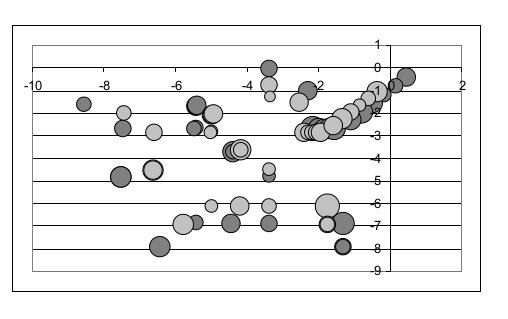
\includegraphics[scale=0.5]{images/movimento_volatil.png}
	\label{fig:volitute_moviment}{\\Fonte: \citeonline{c2009influence}.}
\end{figure}

\section{Intensificação e Diversificação}
\label{sec:intesification_diversification}
Importância da diversificação e diversificação na otimização de problemas dinâmicos e técnicas utilizadas para mante-las.

entropy: \cite{mori2001adaptation}
hamming distance: \cite{rand2005measurements}
memory-of-inertia: \cite{morrison2001measurement}
peak cover: \cite{branke2012evolutionary}
maximun-spread: \cite{goh2009competitive}